\documentclass[conference]{IEEEtran}
\usepackage[utf8]{inputenc}
\usepackage[T1]{fontenc}
\usepackage{lmodern}
\usepackage[english]{babel}
\usepackage{amsmath, amssymb, mathtools}
\usepackage{graphicx}
\usepackage{xcolor}
% REMOVED: \usepackage{hyperref} (The first instance)
\usepackage{algorithm}
\usepackage[noend]{algpseudocode}
\usepackage{booktabs}
\usepackage{multirow}
\usepackage{siunitx}
\usepackage{enumitem}
\usepackage{float}
\usepackage{placeins}
\usepackage{listings}
\usepackage{flushend} 
\usepackage{caption}
\usepackage{threeparttable}
\usepackage{xurl} % Keep this before hyperref

% Keep this as the very last package
\usepackage[hidelinks]{hyperref} 

\pagenumbering{arabic}
\title{Cost-Sensitive Learning for Myocardial Infarction Mortality Prediction: A Static and Dynamic Ensemble Framework}

\author{
\IEEEauthorblockN{Leonardo Saccotelli}
\IEEEauthorblockA{
Università degli Studi di Bari Aldo Moro \\
Email: l.saccotelli@studenti.uniba.it
}
}


\IEEEtitleabstractindextext{%
\begin{abstract}
In this study, we address the binary classification task of predicting admission-time mortality in myocardial infarction patients using the \textit{Myocardial Infarction Complications} dataset from the UCI repository. Our goal is to compare a non-ensemble baseline, static ensemble models, and dynamic ensemble selection methods in the context of class-imbalanced and cost-sensitive learning. We investigate both learning-level and decision-level strategies, including class-frequency-based weighting, cost-matrix-driven weighting, SMOTE, and Minimum Expected Cost (MEC) prediction. The evaluation protocol is based on repeated stratified 10 $\times$ 10 cross-validation with nested hyperparameter optimization, and performance is assessed using both standard classification metrics and an Average Cost metric reflecting asymmetric penalties for false positives and false negatives. Our results show that explicitly accounting for class imbalance is essential in this task, and that cost-sensitive learning combined with the standard decision rule provides the most reliable overall performance. Among the evaluated models, static ensemble approaches, particularly \texttt{StackingClassifier} and \texttt{XGBClassifier}, achieved the best results, while \texttt{DESKL} emerged as the most competitive dynamic selection method.
\end{abstract}
}%

\begin{document}
\maketitle
\IEEEdisplaynontitleabstractindextext

\section{Introduction} 
Myocardial infarction (MI) remains one of the leading causes of death worldwide, and early risk stratification is crucial for improving clinical decision-making and patient management. In particular, the ability to identify, at hospital admission, patients at higher risk of lethal outcome may support timely interventions and more appropriate allocation of critical care resources. From a machine learning perspective, this prediction task is challenging because clinical tabular datasets often exhibit heterogeneous variables, substantial missingness, limited sample size, and marked class imbalance, all of which can negatively affect the learning process. 

Class imbalance is especially problematic in mortality prediction, where the minority class corresponds to the clinically most important cases. In such settings, standard learning algorithms tend to favor the majority class, which may lead to apparently good global performance but poor identification of high-risk patients. Moreover, not all classification errors have the same practical relevance: predicting survival for a patient who actually belongs to the lethal outcome class is generally more critical than the opposite error. These considerations motivate the adoption of imbalance-aware and cost-sensitive strategies that explicitly account for both the rarity of the minority class and the asymmetric cost of misclassification. 

In this work, we study admission-time mortality prediction on the \textit{Myocardial Infarction Complications} dataset, focusing on a binary lethal-outcome setting. We compare a broad range of predictive approaches, including a non-ensemble baseline, static ensemble models, and dynamic ensemble selection (DES) methods. In parallel, we investigate multiple strategies for handling class imbalance, including class-frequency-based weighting, cost-matrix-driven weighting, and data-level oversampling through SMOTE. We also compare the standard threshold-based decision rule with a Minimum Expected Cost (MEC) policy in order to assess the contribution of cost-sensitive prediction at decision time. 
The main contributions of this study are threefold:

\begin{itemize}
    \item \textbf{Systematic Evaluation:} We provide a systematic comparison of static and dynamic ensemble methods for admission-time MI mortality prediction under a unified experimental protocol.
    \item \textbf{Cost-Sensitive Analysis:} We analyze the impact of learning-level and decision-level cost-sensitive strategies, distinguishing between imbalance-aware weighting, cost-matrix-driven learning, and MEC-based prediction.
    \item \textbf{Asymmetric Metrics:} We evaluate all configurations using both standard classification metrics and a cost-sensitive performance criterion aligned with the asymmetric clinical importance of false negatives and false positives.
\end{itemize}

The remainder of the paper is organized as follows. Section~\ref{sec:related-works} reviews related studies on MI prognosis and class imbalance. Section~\ref{sec:methodology} describes the dataset, preprocessing, imbalance-aware strategies, predictive models, and evaluation protocol. Section~\ref{sec:experiment-setup} presents the experimental settings and evaluation metrics. Section~\ref{sec:results} reports the empirical results, while Section~\ref{sec:discussion} discusses the main findings and limitations. Finally, Section~\ref{sec:conclusions} concludes the paper and outlines future research directions.


\section{Related Work} \label{sec:related-works}
Machine learning has been increasingly applied to myocardial infarction (MI) prognosis and complication prediction. However, clinical tabular datasets often contain missing values, heterogeneous variables, and highly imbalanced outcome distributions. Imbalance is especially critical for mortality prediction, where the lethal outcome represents a minority class, and standard metrics such as accuracy may overestimate real-world clinical utility. Consequently, recent studies based on the Myocardial Infarction Complications dataset have explored different modeling strategies to address these challenges \cite{ghafari2023prediction, vicente2024explainablelightgbmapproachpredicting, NEWAZ2023101361}.

Among the works focused on mortality, Ghafari et al. \cite{ghafari2023prediction} predict fatal acute complications within the first 72 hours after hospitalization. Using recursive feature elimination, they evaluate several traditional algorithms and identify XGBoost as the top performer. Similarly, Vicente et al. \cite{vicente2024explainablelightgbmapproachpredicting} investigate mortality prediction on the same dataset using boosted-tree ensembles, namely XGBoost, LightGBM, and CatBoost. They show that LightGBM achieves the best overall performance without extensive preprocessing and complement their analysis with SHAP-based interpretability. Although these studies establish strong mortality-oriented baselines, they remain limited to individual learners or a narrow family of tree ensembles.

Newaz et al. \cite{NEWAZ2023101361} explicitly address the class imbalance by predicting early MI complications using admission-time variables. They propose a hybrid strategy that combines resampling with a cost-sensitive XGBoost model. Their results indicate that jointly addressing imbalance and asymmetric misclassification costs outperforms purely sampling-based or purely cost-sensitive alternatives. However, as in previous studies, their framework remains tied to a single boosted model rather than exploring broader ensemble strategies.

Other studies based on the same dataset broaden the prediction task beyond mortality. Baidya and Gupta \cite{Baidya2024} focus on predicting heart failure and atrial fibrillation. Elashmawi et al. \cite{Elashmawi2024} reframe the problem as multi-target classification, comparing Binary Relevance and Classifier Chains for concurrent MI complications. More recently, Makhmudov et al. \cite{Makhmudov2025} propose a multitask deep learning model to jointly predict multiple complications and mortality causes. While these contributions highlight the richness of the dataset, they target broader multi-complication scenarios rather than optimizing for a focused, admission-time lethal outcome.

Further evidence supports the need for specialized cost-sensitive pipelines. For example, Zheng et al. \cite{zheng2024cost} propose a cost-sensitive deep neural network combined with threshold moving for mortality prediction in acute MI patients with hypertension. Although evaluated on an external cohort with a different pipeline, this work reinforces the need for imbalance-aware designs in MI mortality modeling.

Overall, the literature demonstrates a growing interest in MI risk modeling and an increasing awareness of the class imbalance problem. However, current research still lacks a unified comparison that jointly investigates static ensembles, dynamic ensemble learning, and cost-sensitive techniques for admission-time lethal outcome prediction.

\section{Methodology} \label{sec:methodology}
\subsection{Dataset Description}
This study uses the Myocardial Infarction Complications dataset, a publicly available benchmark released through the UCI Machine Learning Repository and the University of Leicester Figshare archive \cite{golovenkin2020myocardial}. The database was originally collected at the Krasnoyarsk Interdistrict Clinical Hospital, Russia, between 1992 and 1995, and was made publicly available in 2020. It contains 1700 patient records and 124 total columns, including 1 identifier, 111 input features, and 12 target variables describing possible MI complications and lethal outcomes. 

The input features encompass demographic characteristics (\texttt{AGE}, \texttt{SEX}), medical history information (e.g., \texttt{INF\_ANAM}, \texttt{GB}, \texttt{ZSN}), cardiac and blood pressure measurements (e.g., \texttt{S\_AD\_KBRIG}, \texttt{D\_AD\_KBRIG}, \texttt{DLIT\_AG}), laboratory values and electrolyte levels (e.g., \texttt{K\_BLOOD}, \texttt{NA\_BLOOD}), electrocardiogram findings (e.g., \texttt{ant\_im}, \texttt{lat\_im}, \texttt{ritm\_ecg\_p\_01}, \texttt{MP\_TP\_POST}) and treatment-related variables (e.g., \texttt{NA\_KB}, \texttt{LID\_KB}, \texttt{NITR\_S}). 

The target variables include 11 complication-related variables, covering events such as atrial fibrillation (\texttt{FIBR\_PREDS}), supraventricular tachycardia (\texttt{PREDS\_TAH}), ventricular tachycardia (\texttt{JELUD\_TAH}), and other post-MI complications. Additionally, the variable \texttt{LET\_IS} records lethal outcomes associated with MI, including causes such as cardiogenic shock, pulmonary edema, and myocardial rupture. Finally, the dataset was designed to support prediction at different stages of hospitalization, specifically at admission, after 24 hours, after 48 hours, and after 72 hours.

\subsection{Exploratory Data Analysis (EDA)}
We conducted an exploratory data analysis (EDA) to assess data quality and examine the main characteristics of the dataset. In particular, we analyzed missing values, duplicate records, class imbalance, and variable distributions to inform subsequent preprocessing stages. At the row level, all 1,700 records lack at least one value, with an average missing data rate of 7.64\%. At the column level, seven input features exceed a 30\% missing rate. This confirms the presence of features with low, moderate, and very high missing value proportions. Finally, the dataset does not contain duplicate records.

The analysis focused on both numeric and categorical features. Some numeric features, such as \texttt{AGE}, \texttt{S\_AD\_KBRIG}, \texttt{S\_AD\_ORIT}, and \texttt{NA\_BLOOD}, exhibited relatively regular and approximately symmetric distributions. In contrast, several laboratory-related variables (e.g., \texttt{ALT\_BLOOD}, \texttt{AST\_BLOOD}) were clearly right-skewed with high-value outliers, suggesting the potential need for normalization. Furthermore, the Pearson correlation analysis in Figure \ref{fig:corr-heatmap} indicates that some groups of variables carry partially overlapping information. Systolic and diastolic blood pressure variables exhibited strong positive correlations, while most remaining numerical features showed weak or moderate linear correlations.

\begin{figure}[h]
    \centering
    
\includegraphics[width=\linewidth]{figures/correlation_matrix.png}
    \caption{Correlation heatmap among numeric features.}
    \label{fig:corr-heatmap}
\end{figure}

For categorical features, frequency distributions across nominal and ordinal variables informed our preprocessing pipeline, guiding the use of one-hot or ordinal encoding based on feature semantics. Many binary clinical indicators showed marked imbalances; for example, \texttt{SIM\_GIPERT} was heavily dominated by the \texttt{NO} category (96.18\%), whereas \texttt{SEX} was more moderately imbalanced (\texttt{FEMALE}: 37.35\%, \texttt{MALE}: 62.65\%). General nominal and ordinal features likewise displayed heterogeneous distributions, with patient frequencies often concentrating heavily in the lowest categories (e.g., 62.35\% of patients in level 0 for \texttt{INF\_ANAM}).

A similar imbalance pattern emerged for the complication and lethal outcome targets. Most complications were dominated by the negative class, with positive occurrences ranging from just 1.18\% (\texttt{PREDS\_TAH}) up to 23.18\% (\texttt{ZSN}). The lethal outcome variable \texttt{LET\_IS} was likewise strongly skewed toward the \texttt{ALIVE} class (84.06\%), with individual lethal subclasses accounting for very small fractions of the data (0.71\% to 6.47\%). Overall, this confirmed that both predictors and target variables exhibit highly imbalanced distributions.

The insights obtained through this initial exploration helped shape subsequent decisions regarding feature engineering, model selection, and cost-sensitive strategies.

\subsection{Data Cleaning and Preprocessing}
The original Myocardial Infarction Complications dataset supports prediction at multiple time points during hospitalization. In this study, we focused exclusively on admission-time prediction in the intensive care unit (ICU). Accordingly, we excluded all input features not available at admission, namely \texttt{R\_AB\_1\_n}, \texttt{R\_AB\_2\_n}, \texttt{R\_AB\_3\_n}, \texttt{NA\_R\_1\_n}, \texttt{NA\_R\_2\_n}, \texttt{NA\_R\_3\_n}, \texttt{NOT\_NA\_1\_n}, \texttt{NOT\_NA\_2\_n}, and \texttt{NOT\_NA\_3\_n}.

Among the original target variables, we removed all complication-related targets (\texttt{FIBR\_PREDS}, \texttt{PREDS\_TAH}, \texttt{JELUD\_TAH}, \texttt{FIBR\_JELUD}, \texttt{A\_V\_BLOK}, \texttt{OTEK\_LANC}, \texttt{RAZRIV}, \texttt{DRESSLER}, \texttt{ZSN}, \texttt{REC\_IM}, and \texttt{P\_IM\_STEN}) and retained only the lethal outcome variable \texttt{LET\_IS}. The retained variable \texttt{LET\_IS} was then converted into a binary endpoint, where class \texttt{0} corresponds to \texttt{ALIVE} and class \texttt{1} corresponds to \texttt{DEAD}; the positive class was obtained by collapsing all specific causes of death into a single category. The resulting target distribution is imbalanced, with 84.06\% of patients belonging to the \texttt{ALIVE} class and 15.94\% of patients belonging to the \texttt{DEAD} class, as shown in Figure~\ref{fig:let_is-dist}.

Given the extent of missing data highlighted during the exploratory analysis, we applied a two-level cleaning strategy. First, at the row level, we removed all records with more than 20\% missing values, reducing the dataset from 1700 to 1572 observations. Second, at the column level, we removed all input variables with more than 30\% missing values. The final dataset consisted of 1572 rows and 98 columns, including the identifier column and the binary target variable.

\begin{figure}[h]
    \centering
    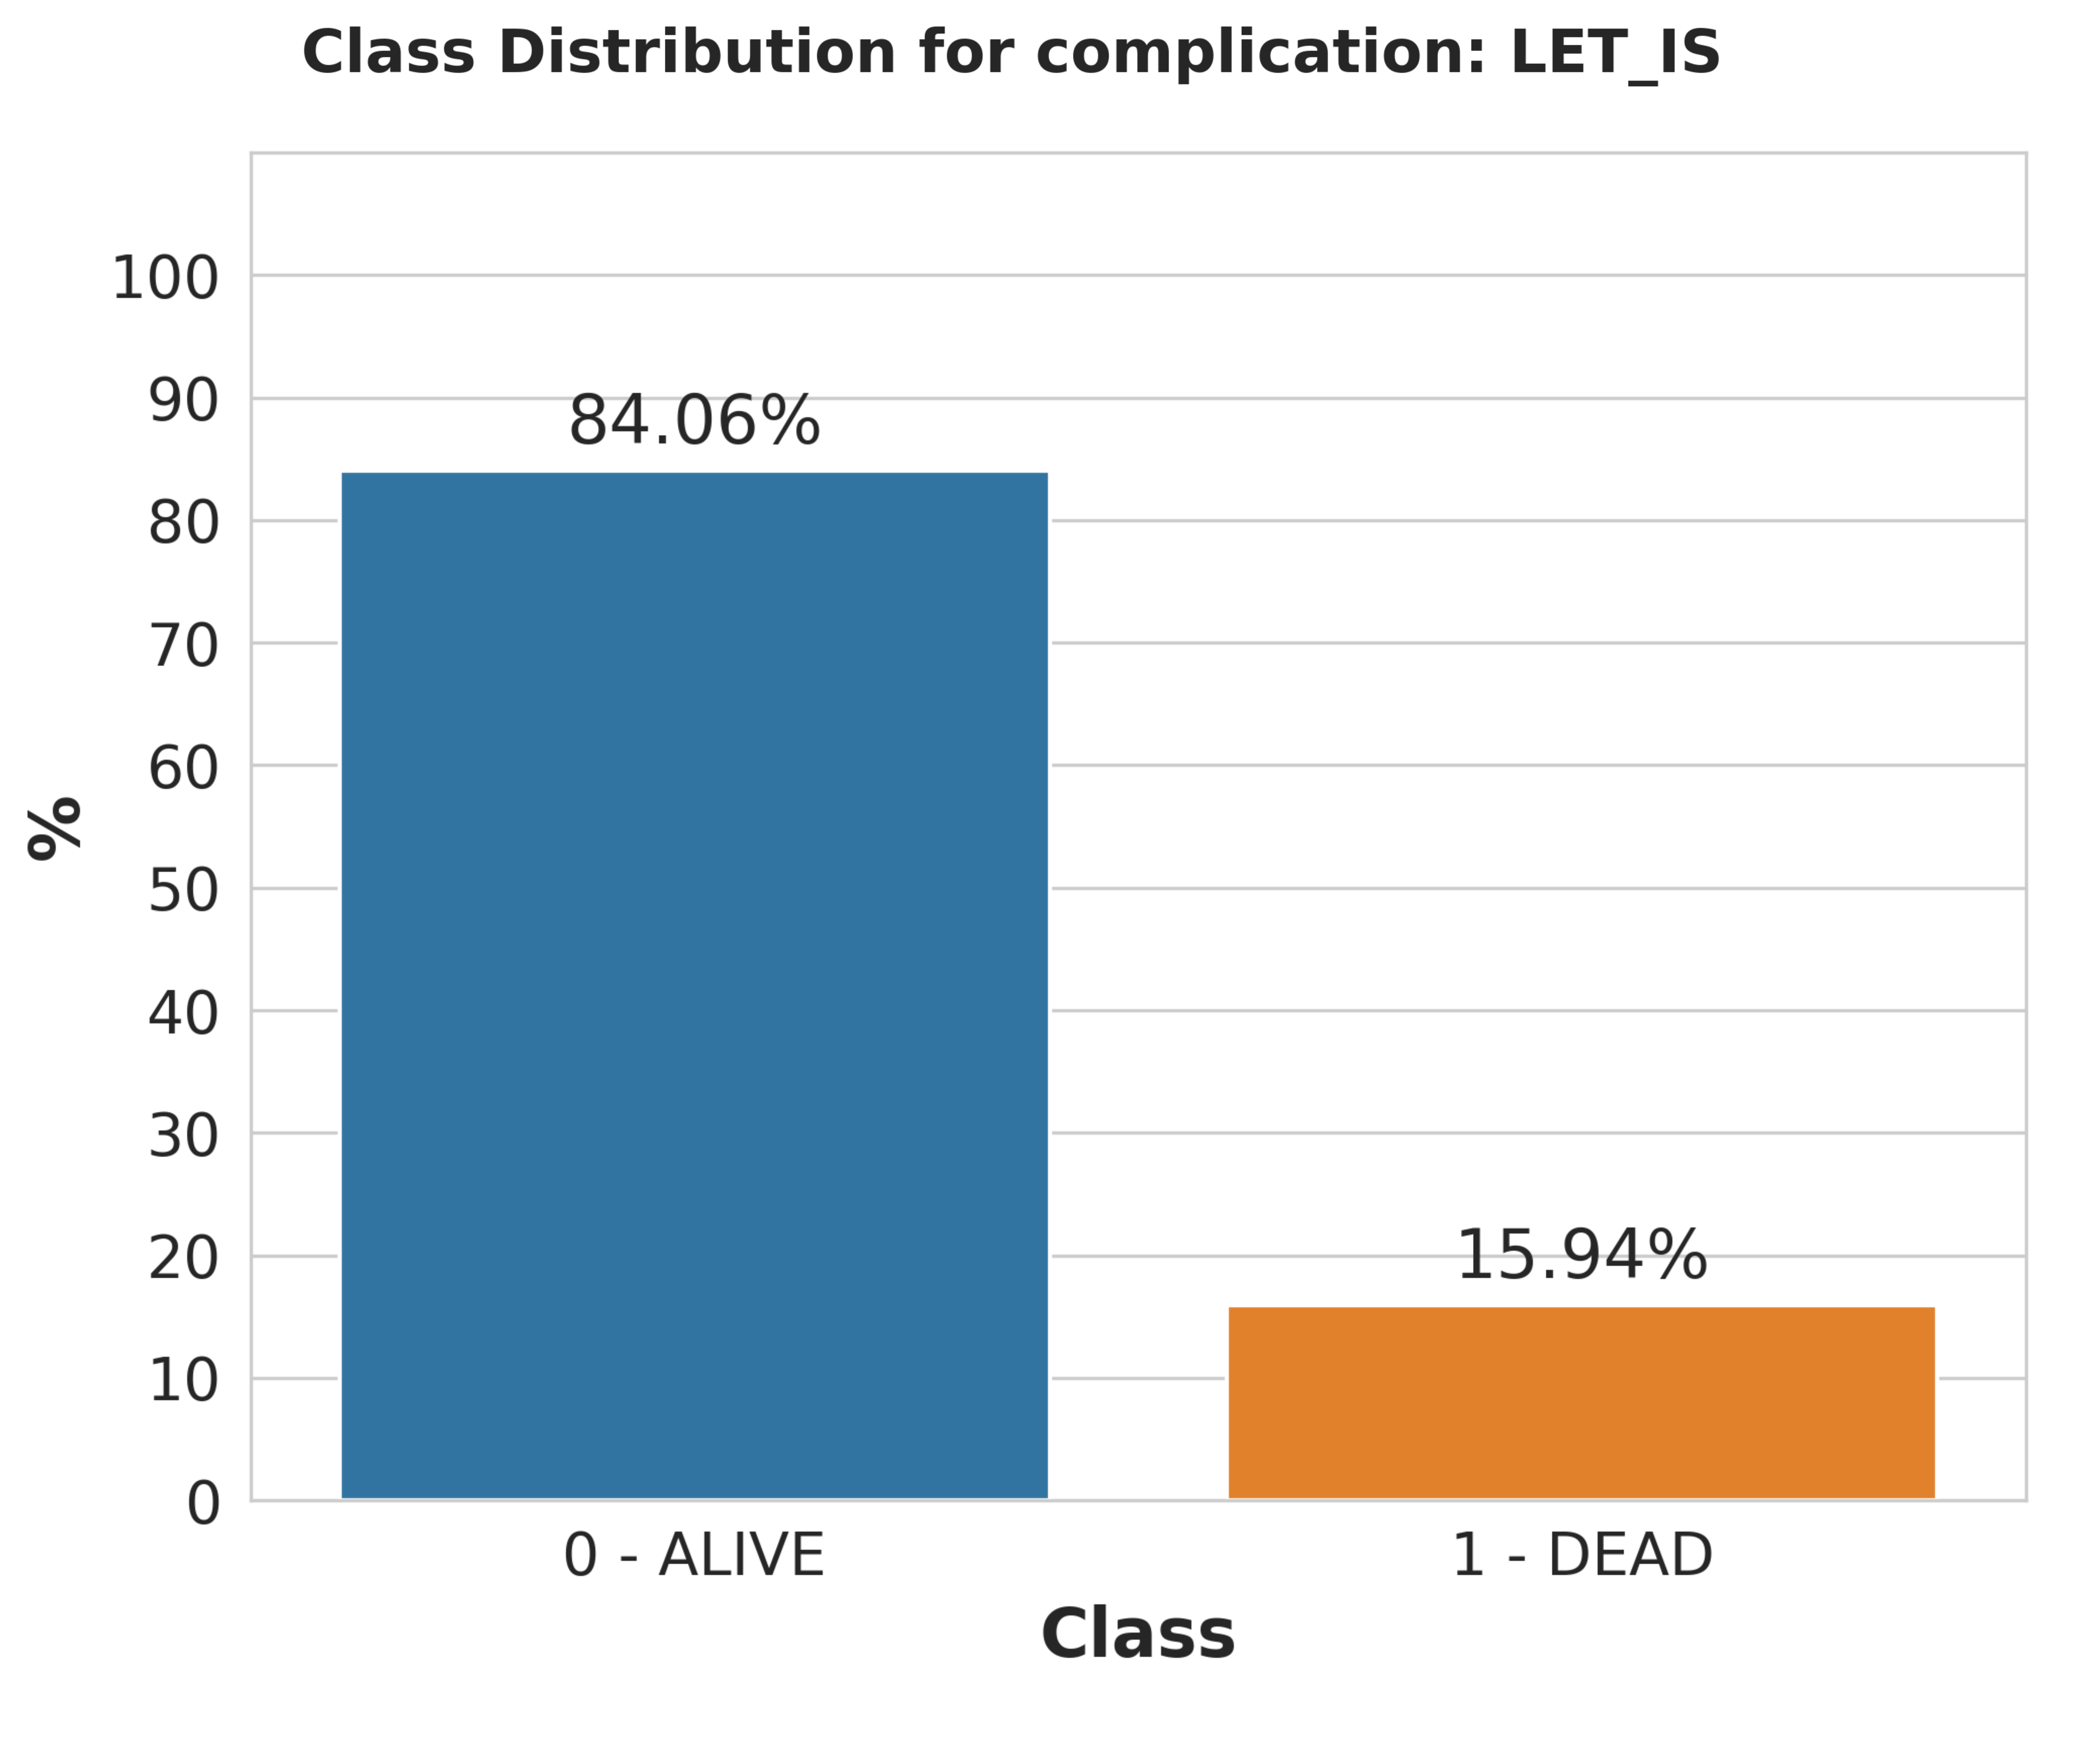
\includegraphics[width=\linewidth]{figures/Class_imbalance.png}
    \caption{Distribution of the target variable \texttt{LET\_IS}.}
    \label{fig:let_is-dist}
\end{figure}

After data cleaning, the remaining features were processed through a feature-type-specific preprocessing pipeline, with imputation, transformation, and encoding defined according to the nature of each feature:

\begin{itemize}
    \item \textbf{Right-skewed numerical features} (e.g., \texttt{L\_BLOOD}, \texttt{ALT\_BLOOD}, \texttt{AST\_BLOOD}, \texttt{ROE}, and \texttt{K\_BLOOD}): Imputed using the median, transformed with \texttt{log1p} to mitigate skewness, and standardized using \texttt{StandardScaler}.

    \item \textbf{Approximately normal numerical features} (e.g., \texttt{AGE}, \texttt{S\_AD\_ORIT}, \texttt{D\_AD\_ORIT}, and \texttt{NA\_BLOOD}): Imputed using the median and directly standardized using \texttt{StandardScaler}.

    \item \textbf{Categorical nominal features} (e.g., \texttt{IBS\_POST}): Imputed using the mode and encoded through \texttt{OneHotEncoder}.

    \item \textbf{Categorical binary features}: Imputed using the mode and retained as binary indicators through \texttt{LabelEncoder}.

    \item \textbf{Categorical ordinal features} (e.g., \texttt{INF\_ANAM}, \texttt{STENOK\_AN}, \texttt{FK\_STENOK}, and \texttt{GB}): Imputed using the mode and encoded according to their natural order through \texttt{OrdinalEncoder}.

    \item \textbf{Categorical partially ordered features} (\texttt{ZSN\_A}): Because its clinical semantics cannot be represented by a single strictly monotonic scale, this feature was imputed using the mode and then transformed into two derived features through a custom partial-order mapping designed to preserve its bidimensional severity structure.
\end{itemize}

Feature selection was performed within the training pipeline using \texttt{SelectKBest} with mutual information as the scoring criterion. The number of retained features, \texttt{k}, was treated as a tunable hyperparameter and searched from 5 up to all available features. 

Importantly, imputation, transformation, and feature selection were all embedded in the training pipeline; therefore, every statistic required by these steps was estimated exclusively on the training set and then applied to the corresponding validation and test partitions, thereby preventing data leakage.

\subsection{Imbalance-Aware and Cost-Sensitive Strategies}
Class imbalance is a critical issue in myocardial infarction mortality prediction because standard learning algorithms tend to favor the majority class, leading to suboptimal recognition of minority-class instances. In the present setting, this limitation is particularly relevant because the minority class corresponds to patients with lethal outcomes, for whom misclassification may have more severe clinical consequences than errors on the majority class \cite{Araf2024}.

For this reason, we considered dedicated strategies to mitigate imbalance and account for asymmetric misclassification costs at both the learning and decision levels.

\subsubsection{Learning-Level Strategies for Imbalanced Classification}

At the learning level, we considered three complementary strategies to address class imbalance:

\begin{itemize}
    \item \textbf{Data-level strategy (SMOTE).}  
    We adopted the Synthetic Minority Oversampling Technique (SMOTE) to increase the representation of the minority class in the training data through the generation of synthetic minority-class samples. This strategy was applied exclusively to the training partition to prevent data leakage.

    \item \textbf{Algorithm-level strategy (class-frequency-based weighting).}  
    For models supporting internal weighting mechanisms, class imbalance was handled through class-frequency-based weighting schemes, such as \texttt{class\_weight="balanced"} or equivalent positive-class scaling parameters (e.g., \texttt{scale\_pos\_weight}). In this setting, the contribution of minority-class instances to the optimization process is increased according to the empirical class distribution, without modifying the original feature space.

    \item \textbf{Cost-sensitive learning strategy.}  
    In addition to class-frequency-based weighting, we implemented a cost-sensitive learning setting in which the weights assigned during training were guided by a specific cost matrix. Thus, unlike standard imbalance-aware weighting, which compensates for the underrepresentation of the minority class, cost-sensitive weighting explicitly reflects the higher clinical severity of false negatives relative to false positives by assigning greater importance to errors involving the \texttt{DEAD} class.
\end{itemize}

The adopted cost matrix is reported in Table~\ref{tab:cost-matrix}. In our setting, false negatives were assigned a substantially higher penalty than false positives, reflecting the greater clinical cost of predicting survival for a patient who actually belongs to the lethal outcome class.

\begin{table}[h]
    \centering
    \caption{Cost matrix adopted for cost-sensitive learning and decision-making.}
    \label{tab:cost-matrix}
    \begin{threeparttable}
        \begin{tabular}{clcc}
            \toprule
            & & \multicolumn{2}{c}{\textbf{Predicted Class}} \\
            \cmidrule(lr){3-4}
            & & \textbf{ALIVE (0)} & \textbf{DEAD (1)} \\
            \midrule
            \multirow{2}{*}{{\textbf{Actual Class}}} 
            & \textbf{ALIVE (0)} & TN = 0 & FP = 1 \\
            & \textbf{DEAD (1)}  & FN = 10 & TP = 0 \\
            \bottomrule
        \end{tabular}
    \end{threeparttable}
\end{table}

\subsubsection{Decision-Level Cost-Sensitive Prediction}

At the decision level, we considered two alternative prediction rules. The first corresponds to the standard threshold-based decision rule, in which a sample is assigned to the positive class whenever the predicted probability of \texttt{DEAD} is greater than or equal to 0.5. This rule does not explicitly account for asymmetric misclassification costs and was therefore used as the default decision baseline.

In addition to the standard thresholding rule, we applied a \textit{Minimum Expected Cost} (MEC) decision rule \cite{elkan2001}. Let \(P(y=k \mid x)\) denote the predicted posterior probability for class \(k\) given input \(x\), and let \(C_{k,c}\) denote the cost of predicting class \(c\) when the true class is \(k\). The predicted class \(\hat{y}\) is then selected as the one minimizing the expected misclassification cost:

\[
\hat{y} = \arg\min_{c} \sum_{k} P(y=k \mid x)\, C_{k,c}.
\]

Under this rule, each prediction is not chosen solely on the basis of the highest posterior probability, but rather on the class associated with the lowest expected decision cost according to Table~\ref{tab:cost-matrix}. This allows the decision process to explicitly reflect the asymmetric clinical relevance of false negatives and false positives.

It is important to emphasize that the MEC rule was treated as a post-hoc cost-sensitive prediction strategy and was therefore kept conceptually distinct from learning-level imbalance handling. In other words, while SMOTE, class-frequency-based weighting, and cost-sensitive learning modify the training process itself, MEC only changes the final decision rule applied to model outputs. This distinction was maintained to preserve methodological clarity and to isolate the respective effects of training-level and decision-level strategies during evaluation.

\subsection{Predictive Models}
To evaluate predictive performance on the ICU admission-time mortality task, we considered a set of predictive models spanning a simple non-ensemble baseline as well as several static and dynamic ensemble paradigms. This design enables the comparison of progressively more expressive approaches, ranging from a linear probabilistic classifier to ensemble methods that combine multiple base learners through either fixed aggregation mechanisms or adaptive selection strategies. The hyperparameter search spaces associated with the considered models and tuned model components are summarized in Table~\ref{tab:model-search-space}.

\subsubsection{Baseline Non-Ensemble Model}

As a baseline model, we considered \texttt{LogisticRegression} (LR). This classifier provides a simple and interpretable probabilistic reference for the mortality prediction task, allowing us to assess the benefit of more complex ensemble-based approaches relative to a standard linear model. The fixed configuration was set to \texttt{solver="liblinear"}, \texttt{penalty="l2"}, and \texttt{max\_iter=1000}.

\subsubsection{Static Ensemble Models}
We considered four static ensemble models, each representing a different aggregation paradigm:

\begin{itemize}

\item \textbf{Random Forest.} \texttt{RandomForestClassifier} (RF) was adopted as a bagging-based ensemble of decision trees. By aggregating multiple trees trained on bootstrap samples and random subsets of features, RF provides a robust non-linear model that is well suited to tabular clinical data. The fixed configuration was set to \texttt{criterion="gini"} and \texttt{bootstrap=True}.

\item \textbf{XGBoost.} \texttt{XGBClassifier} (XGB) was adopted as a tree-based boosting ensemble model. Unlike bagging methods, boosting constructs the ensemble sequentially, with each new learner focusing on correcting the errors of the previous ones. This makes XGB particularly effective for capturing complex interactions in structured tabular datasets. The fixed configuration was set to \texttt{objective="binary:logistic"} and \texttt{eval\_metric="logloss"}.

\item \textbf{Voting Classifier.}  
We considered a heterogeneous static ensemble based on \texttt{VotingClassifier} (Voting), combining RF, XGB, and \texttt{SGDClassifier} (SGD) as base learners. Predictions were aggregated using soft voting, meaning the final class prediction was based on the average predicted probabilities produced by the individual models. Uniform weights were assigned to all base learners. Importantly, the constituent learners were re-instantiated and optimized within the ensemble-specific pipeline, preserving the same fixed settings and hyperparameter search spaces defined for their standalone counterparts.

\item \textbf{Stacking Classifier.}  
We also considered a heterogeneous \texttt{StackingClassifier} (Stacking) combining RF, XGB, and SGD as first-level learners. Their outputs were then combined by a LR meta-estimator. The meta-model was trained using cross-validated predictions of the base learners with \texttt{cv=3}, allowing the second-level learner to exploit complementary predictive patterns captured by the first-level models. As with the Voting ensemble, the constituent learners were re-instantiated and optimized within the ensemble-specific pipeline, while preserving the same fixed settings and hyperparameter search spaces defined for their standalone counterparts.
\end{itemize}

\subsubsection{Dynamic Ensemble Selection}

Dynamic Ensemble Selection (DES) methods select, for each query sample, the subset of classifiers that is estimated to be the most competent in its local context, rather than relying on a fixed ensemble for all instances. According to the taxonomy proposed in \cite{CRUZ2018195}, a DES system typically involves three key elements: the definition of a region of competence around the query sample, the estimation of the local competence of the classifiers in the pool, and the dynamic selection of the ensemble used for the final prediction. 

In our setting, the DES models operated on a classifier pool generated by a \texttt{BaggingClassifier} with \texttt{DecisionTreeClassifier} as the base estimator, while competence estimation was performed on a dedicated dynamic selection dataset (DSEL). We considered three representative DES approaches spanning different competence estimation paradigms identified in the literature: an oracle-based method (\texttt{KNORAE}), a probabilistic method (\texttt{DESKL}), and a meta-learning-based method (\texttt{METADES}). All DES models were configured with a neighborhood size of \texttt{k=7}, using a k-nearest neighbors search with Minkowski distance for competence estimation. In addition, all methods used \textit{soft voting} to aggregate the predictions of the selected classifiers.

\begin{itemize} 
\item \textbf{KNORA-E.} \texttt{KNORAE} (\textit{k-Nearest Oracles Eliminate}) is an oracle-based dynamic ensemble selection method. For a given query sample, the algorithm searches its local region of competence (defined via k-nearest neighbors) for "local oracles"--base classifiers that achieve perfect 100\% accuracy on all samples within this neighborhood. Theoretically, if no classifier satisfies this strict condition, the region of competence is progressively reduced by eliminating the farthest neighbor, and the search is restarted until at least one competent classifier is identified. To form the final prediction, the decisions of the selected oracles the predicted probabilities are aggregated by soft voting schema.

\item \textbf{DES-KL.} \texttt{DESKL} is a probabilistic DES method that evaluates competence from an information-theoretic perspective using a potential function model. While the theoretical formulation of DES-KL considers the entire DSEL, practical implementations restrict the computation to a local region of competence to reduce computational overhead. Accordingly, within the k-NN defined neighborhood, it weights each local sample based on its Euclidean distance from the query through a Gaussian potential function. The source of local competence ($C_{src}$) is calculated as the Kullback--Leibler (KL) divergence between the uniform distribution (representing a random guess) and the vector of class supports produced by the classifier. Because KL divergence is strictly non-negative, a sign-flipping mechanism is applied: $C_{src}$ is assigned a positive sign if the base classifier correctly predicted the neighbor, and a negative sign otherwise. The final competence is the distance-weighted sum of these $C_{src}$ values. Classifiers achieving an overall positive competence are selected.

\item \textbf{META-DES.} \texttt{METADES} reformulates dynamic selection as a meta-learning problem. Instead of relying on a single, fixed competence criterion, it extracts multiple sets of meta-features that characterize the behavior of each base classifier. During the meta-training stage, these meta-features are extracted from instances in both the training set and the DSEL to train a dedicated meta-classifier ($\lambda$), implemented as a Multinomial Naive Bayes model. When an unknown query sample is presented, its local meta-features are calculated and fed into this meta-classifier, which outputs a binary meta-class predicting whether a given base classifier is "competent" (1) or "incompetent" (0) for that specific instance. Classifiers with a predicted competence level above a predefined threshold are selected.
\end{itemize}

\begin{table*}[t]
\centering
\caption{Considered models and tuned model components with their associated hyperparameter search spaces.}\label{tab:model-search-space}
\begin{threeparttable}
\begin{tabular}{p{4.5cm} p{12.8cm}}

\toprule
\textbf{Model} & \textbf{Hyperparameter search space} \\

\midrule
\texttt{LogisticRegression} &
\texttt{C} \(\in [10^{-4}, 10^{4})\) (log-uniform); \texttt{tol} \(\in [10^{-5}, 10^{-2})\) (log-uniform); \texttt{fit\_intercept} \(\in \{\texttt{True}, \texttt{False}\}\) \\
\midrule

\texttt{SGDClassifier} &
\texttt{alpha} \(\in [10^{-5}, 10)\) (log-uniform); \texttt{penalty} \(\in \{\texttt{l2}, \texttt{l1}, \texttt{elasticnet}\}\); \texttt{l1\_ratio} \(\in [0, 1)\) \\
\midrule

\texttt{BaggingClassifier} (\texttt{DecisionTreeClassifier} base estimator) &
\texttt{n\_estimators} \(\in [100, 1000)\); \texttt{max\_samples} \(\in [0.5, 0.9)\);
\texttt{max\_depth} \(\in [3, 20)\); \texttt{min\_samples\_split} \(\in [2, 10)\); \texttt{min\_samples\_leaf} \(\in [1, 10)\);  \texttt{max\_leaf\_nodes} \(\in [2, 20)\); \texttt{min\_impurity\_decrease} \(\in [0.0, 0.1)\); \texttt{ccp\_alpha} \(\in [0.0, 0.01)\) \\
\midrule

\texttt{RandomForestClassifier} &
\texttt{n\_estimators} \(\in [100, 1000)\); \texttt{max\_samples} \(\in [0.5, 0.9)\); 
\texttt{max\_features} \(\in \{\texttt{sqrt}, \texttt{log2}, \texttt{None}\}\);
\texttt{max\_depth} \(\in [3, 20)\); \texttt{min\_samples\_split} \(\in [2, 10)\); \texttt{min\_samples\_leaf} \(\in [1, 10)\);  \texttt{max\_leaf\_nodes} \(\in [2, 20)\); \texttt{min\_impurity\_decrease} \(\in [0.0, 0.1)\); \texttt{ccp\_alpha} \(\in [0.0, 0.01)\) \\
\midrule

\texttt{XGBClassifier} &
\texttt{n\_estimators} \(\in [200, 800)\); \texttt{learning\_rate} \(\in [10^{-2}, 0.2)\) (log-uniform); \texttt{max\_depth} \(\in [3, 10)\); \texttt{subsample} \(\in [0.6, 1.0)\); \texttt{colsample\_bytree} \(\in [0.6, 1.0)\); \texttt{gamma} \(\in [0.0, 5.0)\); \texttt{reg\_alpha} \(\in [10^{-4}, 10)\) (log-uniform); \texttt{reg\_lambda} \(\in [10^{-4}, 10)\) (log-uniform); \texttt{min\_child\_weight} \(\in [1, 10)\) \\
\midrule

\texttt{VotingClassifier} &
Base learners (\texttt{RandomForestClassifier}, \texttt{XGBClassifier}, and \texttt{SGDClassifier}) were re-instantiated and optimized within the ensemble-specific pipeline using the same search spaces defined for their standalone counterparts. \\
\midrule

\texttt{StackingClassifier} &
Base learners (\texttt{RandomForestClassifier}, \texttt{XGBClassifier}, and \texttt{SGDClassifier}) were re-instantiated and optimized within the ensemble-specific pipeline using the same search spaces defined for their standalone counterparts; the meta-estimator was kept fixed. \\

\bottomrule
\end{tabular}
\end{threeparttable}
\end{table*}

\subsection{Learning Pipeline and Evaluation Protocol}
The predictive performance of all considered approaches was assessed using a repeated stratified \(10 \times 10\) cross-validation protocol, i.e., 10 repetitions of stratified 10-fold cross-validation. At each outer split, one fold was held out as the test set, while the remaining nine folds were used for model development. This protocol was adopted to obtain a robust performance estimate under repeated train--test partitions while preserving the class distribution in each split. For the baseline non-ensemble model and the static ensemble models, the nine outer training folds were used to perform hyperparameter optimization through \texttt{RandomizedSearchCV} with 30 sampled configurations. Each candidate configuration was evaluated by an inner stratified 5-fold cross-validation procedure. After identifying the best hyperparameter combination, the full pipeline was re-fitted on all nine outer training folds and then evaluated on the held-out outer test fold. This procedure was repeated for every fold and for every repetition of the repeated cross-validation scheme. For the DES methods, the overall outer evaluation protocol remained the same, but the outer training portion was further partitioned to support dynamic selection. Specifically, the nine outer training folds were split into two subsets: \(75\%\) of the data was used as the effective training set for learning the classifier pool, while the remaining \(25\%\) was used as the dynamic selection dataset (DSEL). Hyperparameter optimization for the pool-generation model was again performed on the effective training subset using randomized search with 30 sampled configurations and an inner stratified 5-fold cross-validation. After the best configuration had been selected, the classifier pool was trained on the full \(75\%\) effective training subset, and the DSEL subset was then used to fit the DES mechanism, including the definition of the region of competence and local competence estimation. The fully specified DES model was finally evaluated on the held-out outer test fold. All preprocessing operations were embedded within the training pipeline in order to prevent data leakage. In particular, imputation, feature transformation, feature selection, and optional oversampling through SMOTE were always fitted exclusively on the effective training data of each split. For the baseline and static ensemble models, these steps were therefore learned only from the training folds involved in the current fitting procedure. For the DES approaches, the same steps were fitted only on the \(75\%\) effective training subset used to train the classifier pool, and the learned transformations were subsequently applied to both the DSEL subset and the outer test fold. As a result, no information from the validation, DSEL, or test partitions was used during the fitting of preprocessing or feature-selection steps.

\section{Experiment Setup} \label{sec:experiment-setup}
\subsection{Experimental Settings}

We defined seven experimental settings to compare cost-insensitive, imbalance-aware, and cost-sensitive configurations under a common evaluation protocol. The first setting corresponds to a baseline experiment with no resampling, no class weighting, and the standard decision rule based on a threshold of 0.5.

The remaining settings were organized into three groups. First, we considered a class-frequency-based weighting strategy, implemented through \texttt{class\_weight="balanced"} or the equivalent positive-class scaling mechanism for XGBoost. This configuration was evaluated under both the standard decision rule and the Minimum Expected Cost (MEC) rule. Second, we considered a cost-sensitive learning strategy based on business-rule weights \(\{0:1, 1:10\}\), again evaluated with both the standard decision rule and MEC. Third, we considered a data-level strategy based on SMOTE with \texttt{sampling\_strategy="auto"}, also evaluated under both the standard decision rule and MEC.

Overall, the experimental comparison included: (i) one baseline setting, (ii) two class-frequency-based weighting settings, (iii) two cost-matrix-driven weighting settings, and (iv) two SMOTE-based settings. Whenever MEC was applied, the same cost matrix used in the methodology section was adopted, with false positives assigned cost 1 and false negatives assigned cost 10.

\subsection{Evaluation Metrics}
For each cross-validation fold, we computed a set of standard classification metrics together with a domain-specific cost metric:

\begin{itemize}
\item \textbf{Standard Metrics}: the standard metrics included Accuracy, Precision, Recall, F1-score, and ROC-AUC, in order to assess general discriminative performance. 

\item \textbf{Average Cost per Prediction} (AvgCost), defined as
\[
\text{AvgCost} = \frac{1 \cdot \text{FP} + 10 \cdot \text{FN}}{N},
\]
where FP and FN denote the numbers of false positives and false negatives, respectively, and \(N\) is the total number of predictions. This metric directly reflects the asymmetric penalty structure adopted in the study and was used as the primary criterion for model comparison, with lower values indicating better performance.
\end{itemize}

Moreover, to assess whether the observed differences in AvgCost were statistically significant, we applied the corrected resampled t-test. A significance level of \(\alpha = 0.05\) was adopted, so that \(p < 0.05\) indicated rejection of the null hypothesis of equal performance.

\subsection{Implementation Details}

All experiments were implemented in Python 3.10. The main software libraries used in this study were \texttt{scikit-learn==1.6.1}, \texttt{imbalanced-learn==0.14.0}, and \texttt{DESlib==0.3.7}. The experiments were executed on a Lenovo ThinkPad T14 Gen 4 equipped with an Intel Core i7-1355U processor, 16\,GB of DDR5 RAM, and a 512\,GB PCIe Gen4 SSD. The full implementation is publicly available in the following GitHub repository: \url{https://github.com/LeonardoSaccotelli/Cost-Sensitive-Learning-For-Myocardial-Infarction-Mortality-Prediction}. 

\section{Results} \label{sec:results}
\subsection{Overall Comparative Performance}

Table~\ref{tab:summary} reports the overall ranking of all model variants, sorted by ascending Average Cost. The best-performing configuration was \texttt{StackingClassifier} with cost-sensitive learning and the standard decision rule, achieving an Average Cost of \(0.5024 \pm 0.1150\). This was followed by \texttt{StackingClassifier} with SMOTE and MEC (\(0.5316 \pm 0.0995\)) and \texttt{XGBClassifier} with cost-sensitive learning and the standard decision rule (\(0.5367 \pm 0.1283\)). More generally, the top part of the ranking was dominated by static ensemble models, especially stacking- and boosting-based approaches.

Among the secondary metrics, \texttt{StackingClassifier} with cost-sensitive learning also achieved the highest ROC-AUC (\(0.8697 \pm 0.0389\)), while the best F1-score was obtained by \texttt{XGBClassifier} with balanced weighting and the standard decision rule (\(0.5699 \pm 0.0598\)). The highest accuracy was achieved by the baseline \texttt{StackingClassifier} (\(0.8809 \pm 0.0180\)), but this configuration ranked much lower in terms of Average Cost (\(0.9830 \pm 0.1369\)). This confirms that standard metrics alone do not fully capture the asymmetric clinical objective of the task, and that AvgCost provides a more appropriate criterion for overall model comparison.

\subsection{Effect of Learning-Level Imbalance Handling}

A clear pattern emerging from Table~\ref{tab:summary} is that imbalance-aware learning strategies substantially improved performance relative to the cost-insensitive baseline. For all major model families, the baseline configuration without resampling or weighting was consistently outperformed by at least one imbalance-aware alternative. For example, \texttt{LogisticRegression} improved from \(1.0115 \pm 0.1624\) in the baseline setting to \(0.6206 \pm 0.1527\) with balanced weighting and to \(0.5596 \pm 0.1382\) with cost-sensitive learning under the standard decision rule. Similar improvements were observed for \texttt{RandomForestClassifier}, which decreased from \(1.4174 \pm 0.1098\) in the baseline setting to \(0.7086 \pm 0.1392\) with balanced weighting and to \(0.5562 \pm 0.1069\) with cost-sensitive learning.

Across models, cost-sensitive learning driven by the asymmetric class weights \(\{0:1, 1:10\}\) was the most effective learning-level strategy. It produced the best overall configurations for \texttt{StackingClassifier}, \texttt{XGBClassifier}, \texttt{RandomForestClassifier}, \texttt{LogisticRegression}, and also the best DES result for \texttt{DESKL}. Balanced weighting also improved substantially over the baseline, but in most cases it was inferior to the cost-matrix-driven alternative. SMOTE yielded more mixed results: under the standard decision rule it rarely matched the best weighted settings, although it became competitive when combined with MEC for some models, particularly \texttt{StackingClassifier} and \texttt{XGBClassifier}. Overall, these results indicate that directly modifying the learning objective through class weighting was more effective than purely data-level balancing for this task.

\subsection{Effect of the MEC Decision Rule}

The comparison between the standard threshold-based rule and the MEC decision rule reveals a strong shift in the operating point of the classifiers. MEC consistently pushed recall toward its maximum, often reaching \(1.0000\), but this came at the cost of markedly lower precision and accuracy. This behavior is visible in several MEC configurations that converge to very similar results, typically around an Average Cost of \(0.84\), with recall close to or equal to \(1.0\) and precision close to the prevalence of the positive class.

In quantitative terms, MEC was not uniformly beneficial. For many cost-sensitive and balanced-weighting settings, the standard decision rule produced lower Average Cost than MEC. For instance, \texttt{StackingClassifier} with cost-sensitive learning increased from \(0.5024 \pm 0.1150\) under the standard rule to \(0.8403 \pm 0.0017\) under MEC, and \texttt{LogisticRegression} with balanced weighting increased from \(0.6206 \pm 0.1527\) to \(0.7282 \pm 0.0691\). However, MEC was beneficial in selected cases, especially when combined with SMOTE. The most notable examples are \texttt{StackingClassifier}, which improved from \(0.7614 \pm 0.1683\) with SMOTE + standard to \(0.5316 \pm 0.0995\) with SMOTE + MEC, and \texttt{XGBClassifier}, which improved from \(0.9167 \pm 0.1490\) to \(0.5911 \pm 0.1410\). Therefore, MEC should not be viewed as a uniformly superior rule, but rather as a decision mechanism whose effectiveness depends on the underlying learning-level strategy.

\subsection{Static Ensembles versus DES}

The comparison between static ensembles and dynamic ensemble selection methods shows that the best static models remained superior overall. Static ensemble configurations occupied most of the top positions in the ranking, with \texttt{StackingClassifier}, \texttt{XGBClassifier}, and \texttt{RandomForestClassifier} achieving the lowest Average Cost values. In particular, the best static ensemble, \texttt{StackingClassifier} with cost-sensitive learning and the standard decision rule, outperformed all DES variants.

Among the DES methods, the strongest result was obtained by \texttt{DESKL} with cost-sensitive learning and the standard decision rule, with an Average Cost of \(0.5872 \pm 0.1317\). This performance was competitive with several strong static models, but still inferior to the best stacking and boosting configurations. \texttt{METADES} with cost-sensitive learning and the standard rule also achieved a reasonable result (\(0.6352 \pm 0.1432\)), whereas \texttt{KNORAE} was generally less competitive and remained above \(0.83\) even in its best setting. Overall, the DES results suggest that dynamic selection can provide competitive performance under cost-sensitive learning, but in the present study it did not surpass the strongest static ensemble architectures.

\begin{table*}[h]
    \centering
    \caption{Summary of performance metrics across all model variants, with imbalance strategy and decision threshold explicitly shown. Models are sorted by ascending Average Cost.}
    \label{tab:summary}
    \begin{threeparttable}
        \resizebox{\textwidth}{!}{
        \begin{tabular}{lcc|cccccc}
            \toprule
            \textbf{Model} & \textbf{Imbalance Strategy} & \textbf{Threshold} & \textbf{Average Cost} & \textbf{ROC\_AUC} & \textbf{Accuracy} & \textbf{Precision} & \textbf{Recall} & \textbf{F1} \\
            \midrule
            StackingClassifier & Cost-sensitive & Standard & \textbf{0.5024 $\pm$ 0.1150} & \textbf{0.8697 $\pm$ 0.0389} & 0.7271 $\pm$ 0.0506 & 0.3570 $\pm$ 0.0477 & 0.8402 $\pm$ 0.0711 & 0.4990 $\pm$ 0.0515 \\
            StackingClassifier & SMOTE & MEC & 0.5316 $\pm$ 0.0995 & 0.8615 $\pm$ 0.0412 & 0.6104 $\pm$ 0.0768 & 0.2845 $\pm$ 0.0444 & 0.9012 $\pm$ 0.0721 & 0.4297 $\pm$ 0.0466 \\
            XGBClassifier & Cost-sensitive & Standard & 0.5367 $\pm$ 0.1283 & 0.8631 $\pm$ 0.0361 & 0.7587 $\pm$ 0.0529 & 0.3878 $\pm$ 0.0606 & 0.7945 $\pm$ 0.0907 & 0.5165 $\pm$ 0.0561 \\
            StackingClassifier & Balanced & Standard & 0.5510 $\pm$ 0.1380 & 0.8689 $\pm$ 0.0375 & 0.7971 $\pm$ 0.0348 & 0.4285 $\pm$ 0.0551 & 0.7577 $\pm$ 0.0861 & 0.5453 $\pm$ 0.0579 \\
            RandomForestClassifier & Cost-sensitive & Standard & 0.5562 $\pm$ 0.1069 & 0.8424 $\pm$ 0.0413 & 0.5377 $\pm$ 0.1172 & 0.2569 $\pm$ 0.0438 & 0.9347 $\pm$ 0.0609 & 0.4002 $\pm$ 0.0526 \\
            LogisticRegression & Cost-sensitive & Standard & 0.5596 $\pm$ 0.1382 & 0.8372 $\pm$ 0.0449 & 0.6781 $\pm$ 0.0477 & 0.3136 $\pm$ 0.0398 & 0.8346 $\pm$ 0.0825 & 0.4548 $\pm$ 0.0495 \\
            DESKL & Cost-sensitive & Standard & 0.5872 $\pm$ 0.1317 & 0.8268 $\pm$ 0.0470 & 0.6527 $\pm$ 0.0746 & 0.3004 $\pm$ 0.0485 & 0.8332 $\pm$ 0.0853 & 0.4387 $\pm$ 0.0541 \\
            XGBClassifier & SMOTE & MEC & 0.5911 $\pm$ 0.1410 & 0.8334 $\pm$ 0.0581 & 0.5469 $\pm$ 0.1963 & 0.2768 $\pm$ 0.0837 & 0.9041 $\pm$ 0.0855 & 0.4138 $\pm$ 0.0911 \\
            XGBClassifier & Balanced & Standard & 0.5968 $\pm$ 0.1459 & 0.8688 $\pm$ 0.0363 & 0.8309 $\pm$ 0.0272 & 0.4833 $\pm$ 0.0560 & 0.7023 $\pm$ 0.0934 & \textbf{0.5699 $\pm$ 0.0598} \\
            XGBClassifier & Balanced & MEC & 0.5979 $\pm$ 0.0984 & 0.8682 $\pm$ 0.0355 & 0.4444 $\pm$ 0.1086 & 0.2244 $\pm$ 0.0316 & 0.9706 $\pm$ 0.0417 & 0.3631 $\pm$ 0.0410 \\
            LogisticRegression & Balanced & Standard & 0.6206 $\pm$ 0.1527 & 0.8367 $\pm$ 0.0446 & 0.7687 $\pm$ 0.0350 & 0.3851 $\pm$ 0.0498 & 0.7290 $\pm$ 0.0949 & 0.5023 $\pm$ 0.0585 \\
            LogisticRegression & SMOTE & Standard & 0.6229 $\pm$ 0.1316 & 0.8330 $\pm$ 0.0465 & 0.7648 $\pm$ 0.0381 & 0.3818 $\pm$ 0.0486 & 0.7302 $\pm$ 0.0834 & 0.4993 $\pm$ 0.0525 \\
            VotingClassifier & Cost-sensitive & Standard & 0.6286 $\pm$ 0.1549 & 0.8386 $\pm$ 0.0472 & 0.5637 $\pm$ 0.1763 & 0.2720 $\pm$ 0.0690 & 0.8662 $\pm$ 0.0905 & 0.4068 $\pm$ 0.0785 \\
            METADES & Cost-sensitive & Standard & 0.6352 $\pm$ 0.1432 & 0.8273 $\pm$ 0.0506 & 0.7317 $\pm$ 0.0611 & 0.3526 $\pm$ 0.0588 & 0.7446 $\pm$ 0.1010 & 0.4740 $\pm$ 0.0580 \\
            VotingClassifier & Balanced & Standard & 0.6441 $\pm$ 0.1550 & 0.8533 $\pm$ 0.0418 & 0.7727 $\pm$ 0.0826 & 0.4121 $\pm$ 0.0948 & 0.7097 $\pm$ 0.1192 & 0.5088 $\pm$ 0.0744 \\
            XGBClassifier & Cost-sensitive & MEC & 0.6946 $\pm$ 0.1088 & 0.8639 $\pm$ 0.0380 & 0.3294 $\pm$ 0.1250 & 0.1947 $\pm$ 0.0289 & 0.9833 $\pm$ 0.0340 & 0.3239 $\pm$ 0.0390 \\
            RandomForestClassifier & Balanced & Standard & 0.7086 $\pm$ 0.1392 & 0.8417 $\pm$ 0.0401 & 0.8033 $\pm$ 0.0341 & 0.4287 $\pm$ 0.0645 & 0.6438 $\pm$ 0.0838 & 0.5125 $\pm$ 0.0649 \\
            LogisticRegression & SMOTE & MEC & 0.7164 $\pm$ 0.0726 & 0.8322 $\pm$ 0.0466 & 0.3042 $\pm$ 0.0837 & 0.1868 $\pm$ 0.0184 & 0.9857 $\pm$ 0.0269 & 0.3135 $\pm$ 0.0251 \\
            LogisticRegression & Balanced & MEC & 0.7282 $\pm$ 0.0691 & 0.8367 $\pm$ 0.0448 & 0.2901 $\pm$ 0.0724 & 0.1834 $\pm$ 0.0150 & 0.9873 $\pm$ 0.0265 & 0.3089 $\pm$ 0.0211 \\
            VotingClassifier & SMOTE & Standard & 0.7462 $\pm$ 0.2047 & 0.8420 $\pm$ 0.0414 & 0.7649 $\pm$ 0.0922 & 0.4080 $\pm$ 0.1109 & 0.6443 $\pm$ 0.1733 & 0.4729 $\pm$ 0.0758 \\
            LogisticRegression & Cost-sensitive & MEC & 0.7610 $\pm$ 0.0539 & 0.8382 $\pm$ 0.0463 & 0.2516 $\pm$ 0.0577 & 0.1755 $\pm$ 0.0109 & 0.9912 $\pm$ 0.0245 & 0.2980 $\pm$ 0.0155 \\
            StackingClassifier & SMOTE & Standard & 0.7614 $\pm$ 0.1683 & 0.8639 $\pm$ 0.0383 & 0.8615 $\pm$ 0.0259 & 0.5746 $\pm$ 0.0838 & 0.5665 $\pm$ 0.1098 & 0.5641 $\pm$ 0.0770 \\
            DESKL & Balanced & Standard & 0.7861 $\pm$ 0.1423 & 0.8309 $\pm$ 0.0440 & 0.8265 $\pm$ 0.0341 & 0.4736 $\pm$ 0.0828 & 0.5737 $\pm$ 0.0874 & 0.5150 $\pm$ 0.0723 \\
            VotingClassifier & SMOTE & MEC & 0.8243 $\pm$ 0.0419 & 0.8443 $\pm$ 0.0410 & 0.1780 $\pm$ 0.0447 & 0.1628 $\pm$ 0.0083 & 0.9984 $\pm$ 0.0078 & 0.2799 $\pm$ 0.0119 \\
            StackingClassifier & Balanced & MEC & 0.8349 $\pm$ 0.0251 & 0.8686 $\pm$ 0.0340 & 0.1651 $\pm$ 0.0251 & 0.1607 $\pm$ 0.0050 & \textbf{1.0000 $\pm$ 0.0000} & 0.2768 $\pm$ 0.0072 \\
            VotingClassifier & Balanced & MEC & 0.8354 $\pm$ 0.0181 & 0.8567 $\pm$ 0.0440 & 0.1669 $\pm$ 0.0276 & 0.1608 $\pm$ 0.0046 & 0.9984 $\pm$ 0.0097 & 0.2769 $\pm$ 0.0064 \\
            KNORAE & Balanced & MEC & 0.8375 $\pm$ 0.0337 & 0.7250 $\pm$ 0.0531 & 0.1723 $\pm$ 0.0134 & 0.1610 $\pm$ 0.0036 & 0.9932 $\pm$ 0.0221 & 0.2770 $\pm$ 0.0059 \\
            VotingClassifier & Cost-sensitive & MEC & 0.8389 $\pm$ 0.0072 & 0.8421 $\pm$ 0.0461 & 0.1611 $\pm$ 0.0072 & 0.1599 $\pm$ 0.0022 & \textbf{1.0000 $\pm$ 0.0000} & 0.2757 $\pm$ 0.0032 \\
            KNORAE & Cost-sensitive & MEC & 0.8398 $\pm$ 0.0472 & 0.7405 $\pm$ 0.0538 & 0.1894 $\pm$ 0.0265 & 0.1624 $\pm$ 0.0057 & 0.9797 $\pm$ 0.0280 & 0.2786 $\pm$ 0.0089 \\
            METADES & SMOTE & MEC & 0.8400 $\pm$ 0.0025 & 0.7399 $\pm$ 0.0638 & 0.1600 $\pm$ 0.0025 & 0.1597 $\pm$ 0.0017 & \textbf{1.0000 $\pm$ 0.0000} & 0.2755 $\pm$ 0.0025 \\
            METADES & Balanced & MEC & 0.8403 $\pm$ 0.0017 & 0.8186 $\pm$ 0.0440 & 0.1597 $\pm$ 0.0017 & 0.1597 $\pm$ 0.0017 & \textbf{1.0000 $\pm$ 0.0000} & 0.2754 $\pm$ 0.0025 \\
            METADES & Cost-sensitive & MEC & 0.8403 $\pm$ 0.0017 & 0.8281 $\pm$ 0.0433 & 0.1597 $\pm$ 0.0017 & 0.1597 $\pm$ 0.0017 & \textbf{1.0000 $\pm$ 0.0000} & 0.2754 $\pm$ 0.0025 \\
            DESKL & Balanced & MEC & 0.8403 $\pm$ 0.0017 & 0.8290 $\pm$ 0.0434 & 0.1597 $\pm$ 0.0017 & 0.1597 $\pm$ 0.0017 & \textbf{1.0000 $\pm$ 0.0000} & 0.2754 $\pm$ 0.0025 \\
            DESKL & Cost-sensitive & MEC & 0.8403 $\pm$ 0.0017 & 0.8270 $\pm$ 0.0436 & 0.1597 $\pm$ 0.0017 & 0.1597 $\pm$ 0.0017 & \textbf{1.0000 $\pm$ 0.0000} & 0.2754 $\pm$ 0.0025 \\
            DESKL & SMOTE & MEC & 0.8403 $\pm$ 0.0017 & 0.7888 $\pm$ 0.0477 & 0.1597 $\pm$ 0.0017 & 0.1597 $\pm$ 0.0017 & \textbf{1.0000 $\pm$ 0.0000} & 0.2754 $\pm$ 0.0025 \\
            RandomForestClassifier & Balanced & MEC & 0.8403 $\pm$ 0.0017 & 0.8448 $\pm$ 0.0402 & 0.1597 $\pm$ 0.0017 & 0.1597 $\pm$ 0.0017 & \textbf{1.0000 $\pm$ 0.0000} & 0.2754 $\pm$ 0.0025 \\
            RandomForestClassifier & Cost-sensitive & MEC & 0.8403 $\pm$ 0.0017 & 0.8431 $\pm$ 0.0423 & 0.1597 $\pm$ 0.0017 & 0.1597 $\pm$ 0.0017 & \textbf{1.0000 $\pm$ 0.0000} & 0.2754 $\pm$ 0.0025 \\
            RandomForestClassifier & SMOTE & MEC & 0.8403 $\pm$ 0.0017 & 0.7908 $\pm$ 0.0492 & 0.1597 $\pm$ 0.0017 & 0.1597 $\pm$ 0.0017 & \textbf{1.0000 $\pm$ 0.0000} & 0.2754 $\pm$ 0.0025 \\
            StackingClassifier & Cost-sensitive & MEC & 0.8403 $\pm$ 0.0017 & 0.8687 $\pm$ 0.0370 & 0.1597 $\pm$ 0.0017 & 0.1597 $\pm$ 0.0017 & \textbf{1.0000 $\pm$ 0.0000} & 0.2754 $\pm$ 0.0025 \\
            KNORAE & SMOTE & MEC & 0.8422 $\pm$ 0.0240 & 0.7013 $\pm$ 0.0616 & 0.1664 $\pm$ 0.0172 & 0.1601 $\pm$ 0.0033 & 0.9940 $\pm$ 0.0174 & 0.2758 $\pm$ 0.0050 \\
            RandomForestClassifier & SMOTE & Standard & 0.8492 $\pm$ 0.1704 & 0.7908 $\pm$ 0.0549 & 0.7944 $\pm$ 0.0470 & 0.4050 $\pm$ 0.0853 & 0.5520 $\pm$ 0.1220 & 0.4604 $\pm$ 0.0829 \\
            KNORAE & Cost-sensitive & Standard & 0.8515 $\pm$ 0.1659 & 0.7396 $\pm$ 0.0583 & 0.7382 $\pm$ 0.0397 & 0.3272 $\pm$ 0.0536 & 0.5894 $\pm$ 0.1083 & 0.4180 $\pm$ 0.0646 \\
            DESKL & SMOTE & Standard & 0.8944 $\pm$ 0.1466 & 0.7908 $\pm$ 0.0485 & 0.8155 $\pm$ 0.0423 & 0.4516 $\pm$ 0.1007 & 0.5058 $\pm$ 0.0962 & 0.4692 $\pm$ 0.0770 \\
            METADES & Balanced & Standard & 0.8975 $\pm$ 0.1689 & 0.8199 $\pm$ 0.0463 & 0.8348 $\pm$ 0.0265 & 0.4854 $\pm$ 0.0857 & 0.4902 $\pm$ 0.1070 & 0.4839 $\pm$ 0.0876 \\
            KNORAE & Balanced & Standard & 0.9104 $\pm$ 0.1678 & 0.7337 $\pm$ 0.0575 & 0.7652 $\pm$ 0.0318 & 0.3476 $\pm$ 0.0595 & 0.5297 $\pm$ 0.1056 & 0.4178 $\pm$ 0.0707 \\
            XGBClassifier & SMOTE & Standard & 0.9167 $\pm$ 0.1490 & 0.8322 $\pm$ 0.0565 & 0.8476 $\pm$ 0.0474 & 0.5669 $\pm$ 0.1458 & 0.4680 $\pm$ 0.0997 & 0.4992 $\pm$ 0.0914 \\
            XGBClassifier & None & Standard & 0.9484 $\pm$ 0.1368 & 0.8657 $\pm$ 0.0368 & 0.8766 $\pm$ 0.0185 & 0.6896 $\pm$ 0.1038 & 0.4259 $\pm$ 0.0860 & 0.5214 $\pm$ 0.0799 \\
            StackingClassifier & None & Standard & 0.9830 $\pm$ 0.1369 & 0.8693 $\pm$ 0.0347 & \textbf{0.8809 $\pm$ 0.0180} & 0.7442 $\pm$ 0.1109 & 0.3988 $\pm$ 0.0864 & 0.5131 $\pm$ 0.0842 \\
            KNORAE & SMOTE & Standard & 0.9980 $\pm$ 0.1687 & 0.7037 $\pm$ 0.0562 & 0.7589 $\pm$ 0.0327 & 0.3264 $\pm$ 0.0633 & 0.4733 $\pm$ 0.1065 & 0.3840 $\pm$ 0.0736 \\
            METADES & SMOTE & Standard & 1.0012 $\pm$ 0.1561 & 0.7570 $\pm$ 0.0652 & 0.8157 $\pm$ 0.0297 & 0.4309 $\pm$ 0.0833 & 0.4315 $\pm$ 0.0978 & 0.4265 $\pm$ 0.0785 \\
            LogisticRegression & None & Standard & 1.0115 $\pm$ 0.1624 & 0.8241 $\pm$ 0.0639 & 0.8592 $\pm$ 0.0393 & 0.6126 $\pm$ 0.1310 & 0.3940 $\pm$ 0.1006 & 0.4720 $\pm$ 0.1015 \\
            VotingClassifier & None & Standard & 1.0925 $\pm$ 0.2184 & 0.8557 $\pm$ 0.0394 & 0.8682 $\pm$ 0.0187 & 0.7014 $\pm$ 0.1531 & 0.3314 $\pm$ 0.1433 & 0.4283 $\pm$ 0.1370 \\
            KNORAE & None & Standard & 1.2171 $\pm$ 0.1505 & 0.7166 $\pm$ 0.0654 & 0.8351 $\pm$ 0.0233 & 0.4766 $\pm$ 0.1649 & 0.2678 $\pm$ 0.0978 & 0.3340 $\pm$ 0.1061 \\
            METADES & None & Standard & 1.3920 $\pm$ 0.1403 & 0.7626 $\pm$ 0.0773 & 0.8486 $\pm$ 0.0146 & 0.6062 $\pm$ 0.2867 & 0.1366 $\pm$ 0.0911 & 0.2117 $\pm$ 0.1240 \\
            DESKL & None & Standard & 1.3997 $\pm$ 0.1115 & 0.7928 $\pm$ 0.0840 & 0.8569 $\pm$ 0.0113 & \textbf{0.8045 $\pm$ 0.2820} & 0.1255 $\pm$ 0.0696 & 0.2121 $\pm$ 0.1069 \\
            RandomForestClassifier & None & Standard & 1.4174 $\pm$ 0.1098 & 0.7890 $\pm$ 0.0809 & 0.8559 $\pm$ 0.0111 & 0.7944 $\pm$ 0.3280 & 0.1138 $\pm$ 0.0709 & 0.1938 $\pm$ 0.1124 \\
            \bottomrule
        \end{tabular}
        }
    \end{threeparttable}
\end{table*}


\subsection{Statistical Significance Analysis} 
To assess whether the observed differences in AvgCost were statistically meaningful, we applied the corrected resampled t-test with significance level \(\alpha = 0.05\). The pairwise significance heatmap in Figure~\ref{fig:heatmap-pvalue-all} shows that a large proportion of the comparisons were statistically significant, indicating that the observed ranking is not merely descriptive but reflects substantial differences among the evaluated configurations. The strongest evidence emerged when comparing imbalance-aware strategies against the baseline setting. In particular, the best-performing cost-sensitive configurations with the standard decision rule---most notably \texttt{StackingClassifier}, \texttt{XGBClassifier}, \texttt{RandomForestClassifier}, and \texttt{LogisticRegression}---showed statistically significant improvements over their corresponding baseline variants in many pairwise comparisons. This result confirms that explicitly addressing class imbalance is beneficial not only in terms of numerical performance, but also from a statistical perspective. The statistical analysis also reinforces the role of cost-sensitive learning combined with the standard decision rule as the most effective configuration family in this study. The top-ranked setting, \texttt{StackingClassifier} with cost-sensitive learning and the standard threshold, was significantly better than a large number of alternative configurations, especially baseline settings and several MEC-based variants. A similar pattern was observed for \texttt{XGBClassifier} under the same cost-sensitive configuration, supporting the conclusion that static ensemble models benefited strongly from cost-sensitive learning applied at the training stage. In contrast, many MEC-based configurations did not differ significantly from one another. This is consistent with the quantitative results reported in Table~\ref{tab:summary}, where several MEC variants converged to similar AvgCost values and exhibited nearly identical operating behavior, typically characterized by extremely high recall and low precision. The statistical results therefore suggest that, under the adopted cost matrix, MEC often drove different models toward a comparable decision regime rather than producing clearly separated performance levels. Regarding the DES family, the best result was obtained by \texttt{DESKL} with cost-sensitive learning and the standard decision rule. The heatmap indicates that this configuration was significantly better than several weaker DES and baseline settings, confirming its competitiveness within the dynamic selection family. However, the statistical comparison does not support a systematic advantage of DES methods over the strongest static ensembles. In particular, the best static models remained among the most favorable configurations both numerically and statistically. Overall, the significance analysis supports five conclusions:

\begin{itemize}
    \item imbalance-aware strategies yield significant improvements over the baseline;
    \item cost-sensitive learning combined with the standard decision rule is the most reliable strategy in this study;
    \item MEC does not provide a uniform advantage and often yields similar performance across different models;
    \item Stacking and XGBoost are the most robust static ensemble approaches;
    \item although DES methods, especially \texttt{DESKL}, are competitive, they do not outperform the best static ensemble configurations in the experimental setting.
\end{itemize}

\begin{figure*}[h]
    \centering
    
\includegraphics[width=\textwidth]{figures/corrected_resampled_ttest_average_cost_heatmap.png}
\caption{Pairwise p-value heatmap of the corrected resampled t-test on AvgCost across all evaluated configurations.}
    \label{fig:heatmap-pvalue-all}
\end{figure*}


\section{Discussion and Limitations} \label{sec:discussion}

The results indicate that explicitly addressing class imbalance is essential for admission-time myocardial infarction mortality prediction. In particular, cost-sensitive learning combined with the standard decision rule yielded the most reliable performance, while static ensemble models, especially \texttt{StackingClassifier} and \texttt{XGBClassifier}, achieved the strongest overall results. Dynamic ensemble selection methods were competitive in selected settings, but did not surpass the best static ensemble configurations in the present study.

Despite these findings, several limitations should be acknowledged. First, the dataset is relatively limited in size and originates from an older clinical context, which may reduce the representativeness of the learned patterns with respect to contemporary medical practice. Extending the analysis to larger and more up-to-date cohorts would therefore be an important step toward improving robustness and practical relevance.

Second, the present work focuses exclusively on mortality prediction at admission time. Although this setting is clinically meaningful for early risk stratification, the same framework could be extended to other temporal stages of hospitalization, as well as to the prediction of specific causes of death and non-lethal myocardial infarction complications.

Third, only a limited set of DES models was explored. While the selected methods cover distinct competence-estimation paradigms, they do not exhaust the broader DES literature. A wider comparison involving additional dynamic selection techniques and alternative pool-generation strategies may provide a more complete assessment of the potential of DES in this context.

Finally, threshold calibration was not explicitly investigated beyond the comparison between the standard decision rule and MEC. Since the operating point of the classifier can strongly affect the trade-off between false positives and false negatives, a dedicated study on threshold calibration may further improve cost-sensitive performance.

\section{Conclusions} \label{sec:conclusions}

This study investigated cost-sensitive learning for admission-time myocardial infarction mortality prediction, comparing a non-ensemble baseline, static ensemble models, and dynamic ensemble selection methods under multiple imbalance-aware and cost-sensitive configurations. The results showed that handling class imbalance is crucial in this task, and that cost-sensitive learning combined with the standard decision rule provides the most reliable overall performance. Among the evaluated models, static ensemble approaches, particularly \texttt{StackingClassifier} and \texttt{XGBClassifier}, achieved the best results, while \texttt{DESKL} emerged as the most competitive DES method.

Several directions can be explored in future work. First, the study should be extended to larger and more up-to-date datasets in order to improve generalizability and clinical relevance. Second, a broader set of DES methods and alternative classifier pools should be evaluated. Finally, future research may extend the prediction task beyond binary lethal outcome to include specific causes of death, non-lethal complications, and dedicated threshold calibration strategies.

\bibliographystyle{IEEEtran}
\bibliography{biblio}
\end{document}